% DPF 09 talk on strangeness in nucleon

\documentclass[10pt]{beamer}
\usepackage{amsmath}
\usepackage{mathtools}
\usefonttheme{professionalfonts} % using non standard fonts for beamer
\usefonttheme{serif} % default family is serif
%\documentclass[12pt]{beamerthemeSam.sty}
\usepackage{epsf}
%\usepackage{pstricks}
%\usepackage[orientation=portrait,size=A4]{beamerposter}
\geometry{paperwidth=160mm,paperheight=120mm}
%DT favorite definitions
\def\LL{\left\langle}	% left angle bracket
\def\RR{\right\rangle}	% right angle bracket
\def\LP{\left(}		% left parenthesis
\def\RP{\right)}	% right parenthesis
\def\LB{\left\{}	% left curly bracket
\def\RB{\right\}}	% right curly bracket
\def\PAR#1#2{ {{\partial #1}\over{\partial #2}} }
\def\PARTWO#1#2{ {{\partial^2 #1}\over{\partial #2}^2} }
\def\PARTWOMIX#1#2#3{ {{\partial^2 #1}\over{\partial #2 \partial #3}} }

\def\rightpartial{{\overrightarrow\partial}}
\def\leftpartial{{\overleftarrow\partial}}
\def\diffpartial{\buildrel\leftrightarrow\over\partial}

\def\BI{\begin{itemize}}
\def\EI{\end{itemize}}
\def\BE{\begin{displaymath}}
\def\EE{\end{displaymath}}
\def\BEA{\begin{eqnarray*}}
\def\EEA{\end{eqnarray*}}
\def\BNEA{\begin{eqnarray}}
\def\ENEA{\end{eqnarray}}
\def\EL{\nonumber\\}


\newcommand{\map}[1]{\frame{\frametitle{\textbf{Course map}}
\centerline{\includegraphics[height=0.86\paperheight]{../../map/#1.png}}}}
\newcommand{\wmap}[1]{\frame{\frametitle{\textbf{Course map}}
\centerline{\includegraphics[width=0.96\paperwidth]{../../map/#1.png}}}}

\newcommand{\etal}{{\it et al.}}
\newcommand{\gbeta}{6/g^2}
\newcommand{\la}[1]{\label{#1}}
\newcommand{\ie}{{\em i.e.\ }}
\newcommand{\eg}{{\em e.\,g.\ }}
\newcommand{\cf}{cf.\ }
\newcommand{\etc}{etc.\ }
\newcommand{\atantwo}{{\rm atan2}}
\newcommand{\Tr}{{\rm Tr}}
\newcommand{\dt}{\Delta t}
\newcommand{\op}{{\cal O}}
\newcommand{\msbar}{{\overline{\rm MS}}}
\def\chpt{\raise0.4ex\hbox{$\chi$}PT}
\def\schpt{S\raise0.4ex\hbox{$\chi$}PT}
\def\MeV{{\rm Me\!V}}
\def\GeV{{\rm Ge\!V}}

%AB: my color definitions
%\definecolor{mygarnet}{rgb}{0.445,0.184,0.215}
%\definecolor{mygold}{rgb}{0.848,0.848,0.098}
%\definecolor{myg2g}{rgb}{0.647,0.316,0.157}
\definecolor{abtitlecolor}{rgb}{0.0,0.255,0.494}
\definecolor{absecondarycolor}{rgb}{0.0,0.416,0.804}
\definecolor{abprimarycolor}{rgb}{1.0,0.686,0.0}
\definecolor{Red}           {cmyk}{0,1,1,0}
\definecolor{Grey}           {cmyk}{.7,.7,.7,0}
\definecolor{Blue}          {cmyk}{1,1,0,0}
\definecolor{Green}         {cmyk}{1,0,1,0}
\definecolor{Brown}         {cmyk}{0,0.81,1,0.60}

\usetheme{Madrid}


%AB: redefinition of beamer colors
%\setbeamercolor{palette tertiary}{fg=white,bg=mygarnet}
%\setbeamercolor{palette secondary}{fg=white,bg=myg2g}
%\setbeamercolor{palette primary}{fg=black,bg=mygold}
\setbeamercolor{title}{fg=abtitlecolor}
\setbeamercolor{frametitle}{fg=abtitlecolor}
\setbeamercolor{palette tertiary}{fg=white,bg=abtitlecolor}
\setbeamercolor{palette secondary}{fg=white,bg=absecondarycolor}
\setbeamercolor{palette primary}{fg=black,bg=abprimarycolor}
\setbeamercolor{structure}{fg=abtitlecolor}

\setbeamerfont{section in toc}{series=\bfseries}

%AB: remove navigation icons
\beamertemplatenavigationsymbolsempty
\title[1D kinematics]{
  \textbf {1D kinematics: position, velocity, and acceleration}\\
(and a calculus review)
%\centerline{}
%\centering
%\vspace{-0.0in}
%\includegraphics[width=0.3\textwidth]{propvalues_0093.pdf}
%\vspace{-0.3in}\\
%\label{intrograph}
}

\author[W. Freeman] {Physics 211\\Syracuse University, Physics 211 Spring 2016\\Walter Freeman}

\date{\today}

\begin{document}

\frame{\titlepage}

\frame{\frametitle{\textbf{The beginning: Free fall}}
\large
\begin{center}
My purpose is to set forth a very new science dealing with a very ancient subject. 
There is, in nature, perhaps nothing older than motion, 
concerning which the books written by philosophers are neither few nor small 
nevertheless I have discovered by experiment some properties of it which are worth 
knowing and which have not hitherto been either observed or demonstrated.... 

\bigskip

So far as I know, no one has yet pointed out that the distances traversed, during equal intervals of time, by a body falling from rest, 
stand to one another {\bf in the same ratio as the odd numbers beginning with unity.}
\bigskip
\end{center}
\bigskip
--Galileo Galilei, {\it Dialogues and Mathematical Demonstrations Concerning Two New Sciences}, 1638
}

\frame{\frametitle{\textbf{Announcements}}
\large
\BI
\item{Homework 1 is due next Wednesday (it's posted)}
\item{We won't start using clickers until next week and no clicker questions will be graded until the following week}

\bigskip

\item{Reminders:}
\BI
\large
\item{Course website: \href{https://suphysics211.wikispaces.com/} (updated frequently!)}
\item{Teaching team contact information:}
\BI
\large
\item{Prof. Walter Freeman: wafreema@syr.edu}
\item{Francesco Serafin: fserafinsyr.edu}
\item{Lab questions; sasemper@syr.edu}
\EI
\EI
\EI
}

\frame{\frametitle{\textbf{Announcements}}

\Large

Did someone lose a piece of jewelry? Tell me if you did...

}

\frame{\frametitle{\textbf{``Ask a Physicist''}}
\Large There are a lot of cool things in physics that go beyond mechanics.

\bigskip
\bigskip
\bigskip

\large

If you've got questions you'd like me to address, send them in and I'll answer them!

\normalsize
\BI
\item{What's the Large Hadron Collider for?}
\item{How does a touchscreen work?}
\item{How do 3D movies work?}
\item{What is the Higgs boson?}
\item{How is physics used in video games?}
\item{How does a nuclear bomb work?}
\item{How does a supercomputer work?}
\EI
}




\frame{\frametitle{\textbf{A few syllabus clarifications}}
\BI
\Large
\item{Exams and schedule (on website)}
\BI
\normalsize
\item{There are two exams on each topic}
\item{You may take both, and keep the better grade}
\item{Since six exams is a lot, ``Exam 3; take 2'' is on the date of the final}
\EI
\pause
\large
\item{Yes, this means you get to retake every exam and improve your score}
\item{I want to see everyone succeed; if you learn something eventually, your grade should reflect that}
\EI
}

\frame{\frametitle{\textbf{Homework tips}}
\centerline{\Large Your first homework assignment is due Wednesday.}

\bigskip
\bigskip

\large
\BI
\item{Make use of words, pictures, and algebra (not just algebra!) in your reasoning}
\item{We're interested in how you think, not just the answer}
\item{Physical values need to be given with units (``4 meters'', not ``4'')}
\item{Paper is cheap -- don't cramp yourself!}
\pause
\bigskip
\item{Ask for help -- early and often}
\BI
\item{Email: suphysics211@gmail.com}
\item{Facebook group}
\item{Office hours}
\item{the Physics Clinic}
\item{Recitations}
\item{In class!}
\EI
\EI
}

\frame{\frametitle{\textbf{The beginning: Free fall}}
\centerline{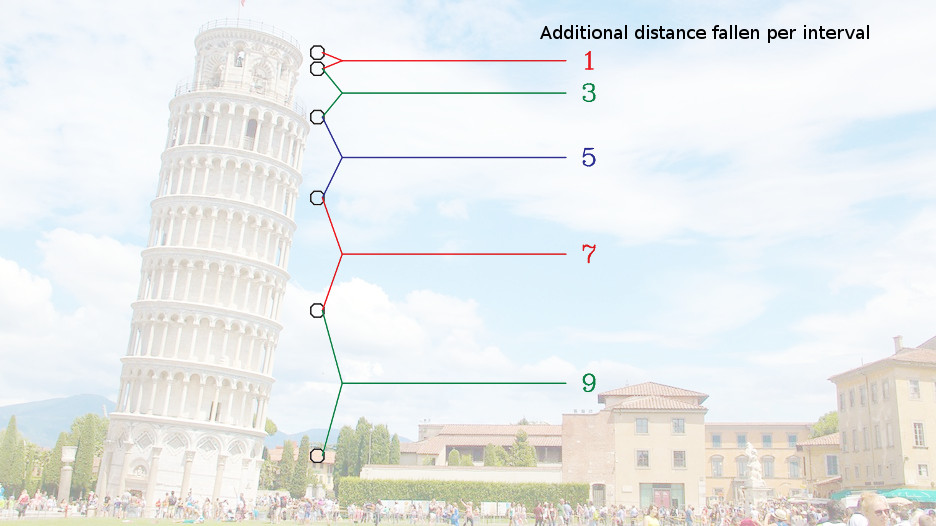
\includegraphics[width=0.8\textwidth]{pisa.jpg}}

\begin{center}
\Large Galileo observed this, but can we explain it?
\end{center}
}

\frame{\frametitle{\textbf{Last time}}
\Large
Constant-velocity motion: $x(t) = x_0 + vt$

\bigskip

\normalsize

\BI

\item{Came from looking at the equation of a line}
\item{We can understand this in a different framework, too:}

\bigskip

\item{\Large Velocity is the {\color{Red} rate of change} of position}
\BI
\item{Graphical representation: Velocity is the slope of the position vs. time graph}
\item{Mathematical language: Velocity is the {\color{Red} derivative} of position}
\EI
\EI

\bigskip
\bigskip

\Large

We know we need to know about acceleration (``F=ma'') -- what is it?

\bigskip
\BI
\item{Acceleration is the {\color{Red} rate of change} of velocity}
\EI
}


\frame{\frametitle{\textbf{Position, velocity, and acceleration}}
\begin{columns}
\column{0.125\textwidth}
\centerline{\Large Position}
\column{0.2\textwidth}
\small
{\color{Red}
\centerline{(derivative of)}
\centerline{rate of change of}
\centerline{$\xleftarrow{\makebox[\textwidth]{}}$}}
\column{0.125\textwidth}
\centerline{\Large Velocity}
\pause
\column{0.2\textwidth}
\small
{\color{Red}
\centerline{(derivative of)}
\centerline{rate of change of}
\centerline{$\xleftarrow{\makebox[\textwidth]{}}$}}
\column{0.15\textwidth}
\centerline{\Large Acceleration}
\end{columns}
}

\frame{\frametitle{\textbf{Kinematics: how does acceleration affect movement?}}
\Large
Newton's law $a = F/m$ tells us that {\it acceleration} -- the second derivative of position -- is what results from forces.\\

\bigskip
\bigskip
\bigskip
\pause
\centerline{All freely falling objects have a constant acceleration downward.}
\bigskip
\bigskip
\centerline{This number is so important we give it a letter: $g = 9.81$ $\rm m/\rm s^2$}
}

\frame{\frametitle{\textbf{A calculus review}}
\begin{center}
If velocity is the rate of change of position, \\
why is the area under the $v$ vs. $t$ curve equal to displacement?
\end{center}

\centerline{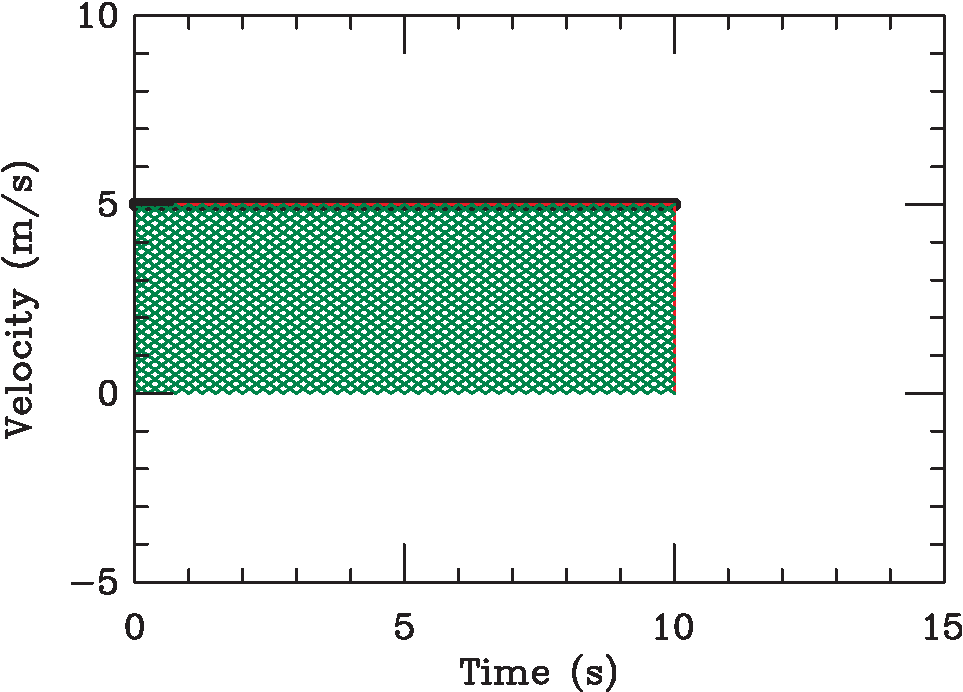
\includegraphics[width=0.7\textwidth]{integral-constant-crop.pdf}}

\bigskip
\bigskip

\centerline{\large We know $\Delta s = vt$. What is that here? What's the area of the shaded region?}

}


\frame{\frametitle{\textbf{A calculus review}}

\centerline{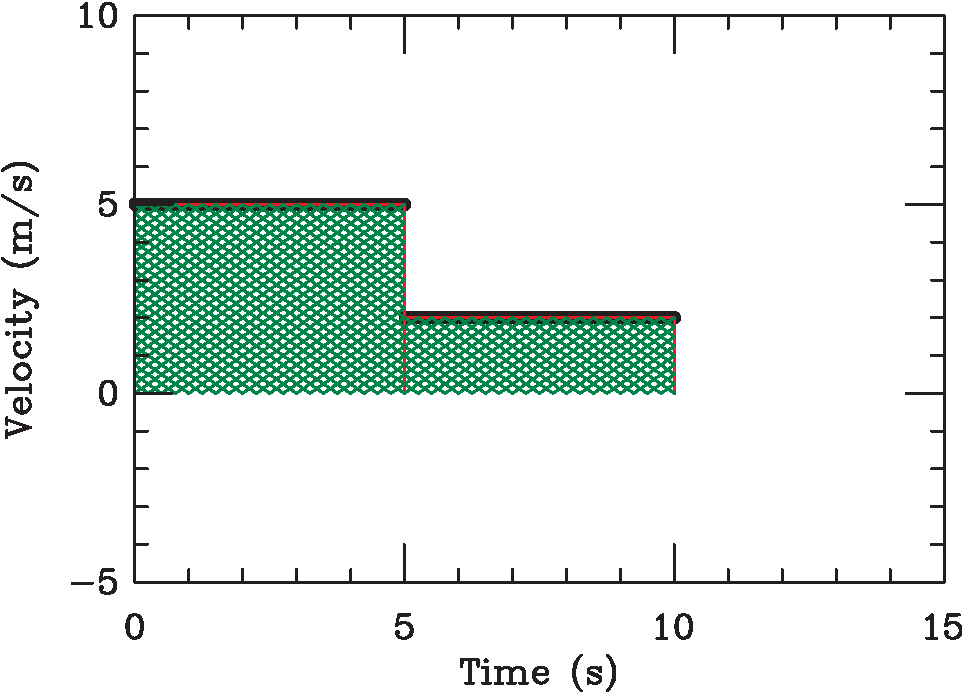
\includegraphics[width=0.6\textwidth]{integral-two-crop.pdf}}

\bigskip
\bigskip
\bigskip

\centerline{\large Now what is $\Delta s$? What is the area of the shaded region?}

}


\frame{\frametitle{\textbf{A calculus review}}

\centerline{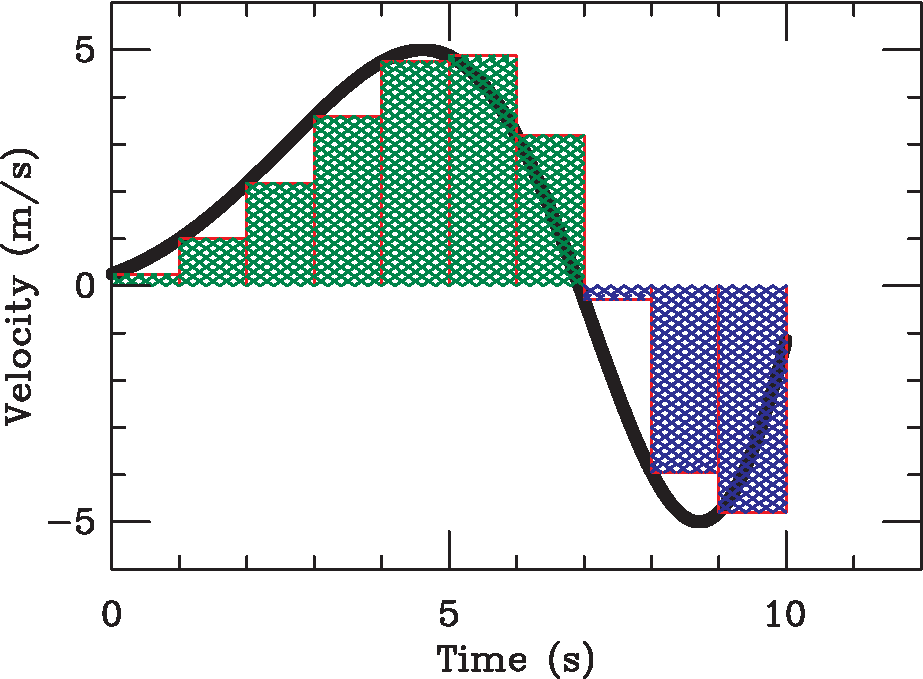
\includegraphics[width=0.6\textwidth]{integral-curve-coarse-crop.pdf}}

\bigskip
\bigskip
\bigskip

\centerline{\large Does this work? How do we fix it?}

}



\frame{\frametitle{\textbf{A calculus review}}

\centerline{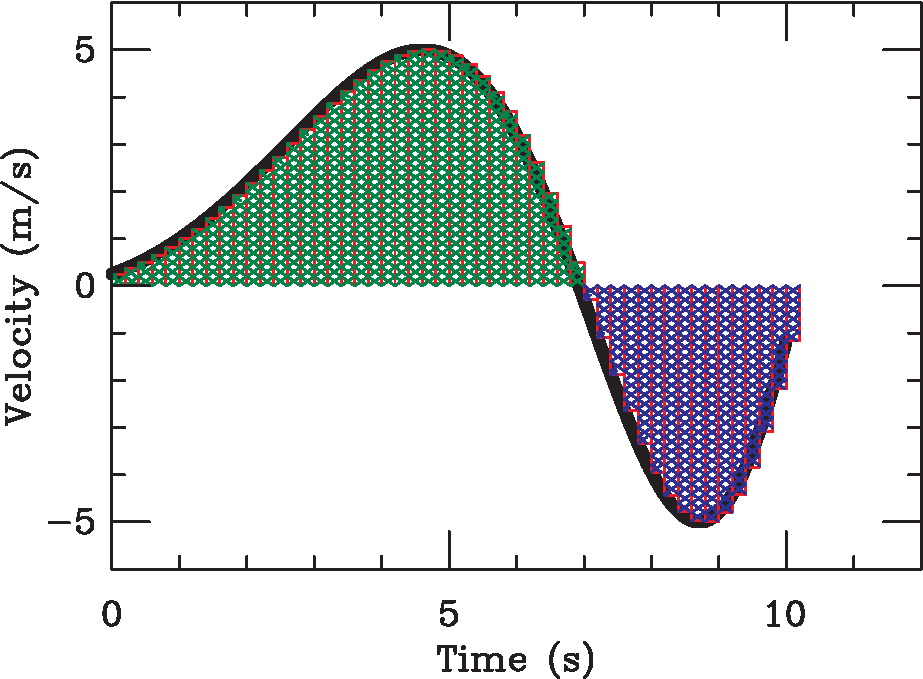
\includegraphics[width=0.6\textwidth]{integral-curve-fine-crop.pdf}}

\bigskip
\bigskip

\centerline{\large The area between the $t$-axis and the velocity curve is the distance traveled.}
\centerline{\large \color{Grey} (The area below the $t$-axis counts negative: ``the thing is going backwards''}
\bigskip
\centerline{\large In calculus notation: $\int v(t)\, dt = \delta x = x(t) - x_0$}

}

\frame{\frametitle{\textbf{Position, velocity, and acceleration}}
\begin{columns}
\column{0.125\textwidth}
\centerline{\Large Position}
\column{0.2\textwidth}
\small
{\color{Red}
\centerline{(derivative of)}
\centerline{rate of change of}
\centerline{$\xleftarrow{\makebox[\textwidth]{}}$}}
{\color{Green}
\color{Green}\centerline{$\xrightarrow{\makebox[\textwidth]{}}$}}
\color{Green}\centerline{area under the curve of}
\color{Green}\centerline{(integral of)}
\column{0.125\textwidth}
\centerline{\Large Velocity}
\pause
\column{0.2\textwidth}
\small
{\color{Red}
\centerline{(derivative of)}
\centerline{rate of change of}
\centerline{$\xleftarrow{\makebox[\textwidth]{}}$}}
{\color{Green}
\color{Green}\centerline{$\xrightarrow{\makebox[\textwidth]{}}$}}
\color{Green}\centerline{area under the curve of}
\color{Green}\centerline{(integral of)}
\column{0.15\textwidth}
\centerline{\Large Acceleration}
\end{columns}
}

\frame{\frametitle{\textbf{Constant acceleration}}
Particularly interesting situation: 
\BI
\item{Free fall (as you saw)}
\item{Any time the force is constant: $F = ma \rightarrow a = F/m$...}
\EI
\bigskip
\pause
Plan of attack:
\BI
\item{We know what the acceleration curve looks like (it's just flat)}
\item{Figure out the area under the acceleration curve to get the velocity curve}
\item{Figure out the area under the velocity curve to get the position curve}
\EI
\pause
\bigskip
\bigskip
\bigskip
\bigskip
Remember the area under the curve of (velocity, acceleration) just gives the {\it change in} (position, velocity) -- \ie initial minus final.

\bigskip
\bigskip

We'll start by assuming $x_0$ and $v_0$ are zero.
}

\frame{\frametitle{\textbf{Constant acceleration}}
\centerline{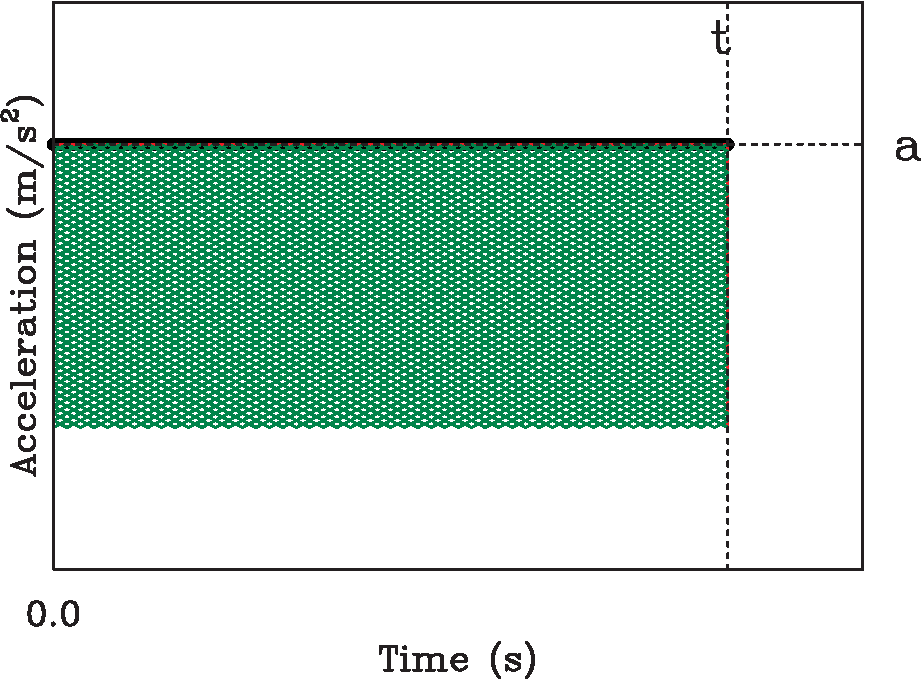
\includegraphics[width=0.6\textwidth]{area-under-a-crop.pdf}}

\bigskip
\bigskip

What's the area under the curve out to time $t$, which gives the change in the velocity -- $\Delta v=v(t) - v_0$?

\pause

\bigskip
\bigskip

\centerline{\Large $v(t) - v_0 = at$, so {\color{Red}$v(t) = at + v_0$}}
}


\frame{\frametitle{\textbf{Same thing again to get position}}
\centerline{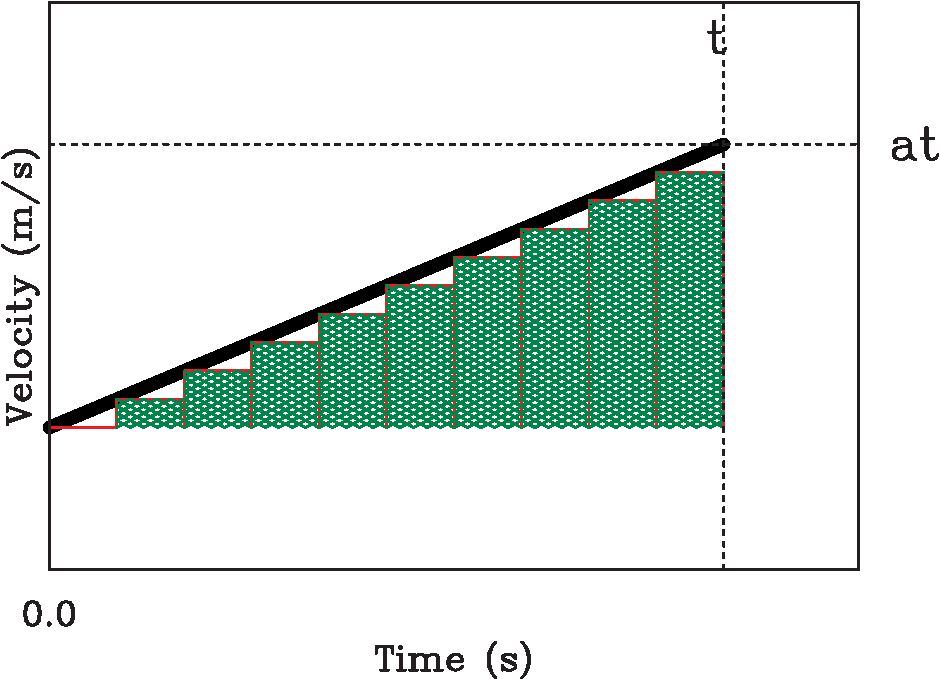
\includegraphics[width=0.6\textwidth]{area-under-v-crop.pdf}}

\bigskip
\bigskip

Now the area under the velocity curve gives the change in position: $\Delta x=x(t) - x_0$?

\pause

\bigskip
\bigskip

\centerline{\Large $x(t) - x_0 = \frac{1}{2}at^2$, thus $x(t) = \frac{1}{2}at + x_0$}
}

\frame{\frametitle{\textbf{Now if $v_0$ is not zero...}}
\centerline{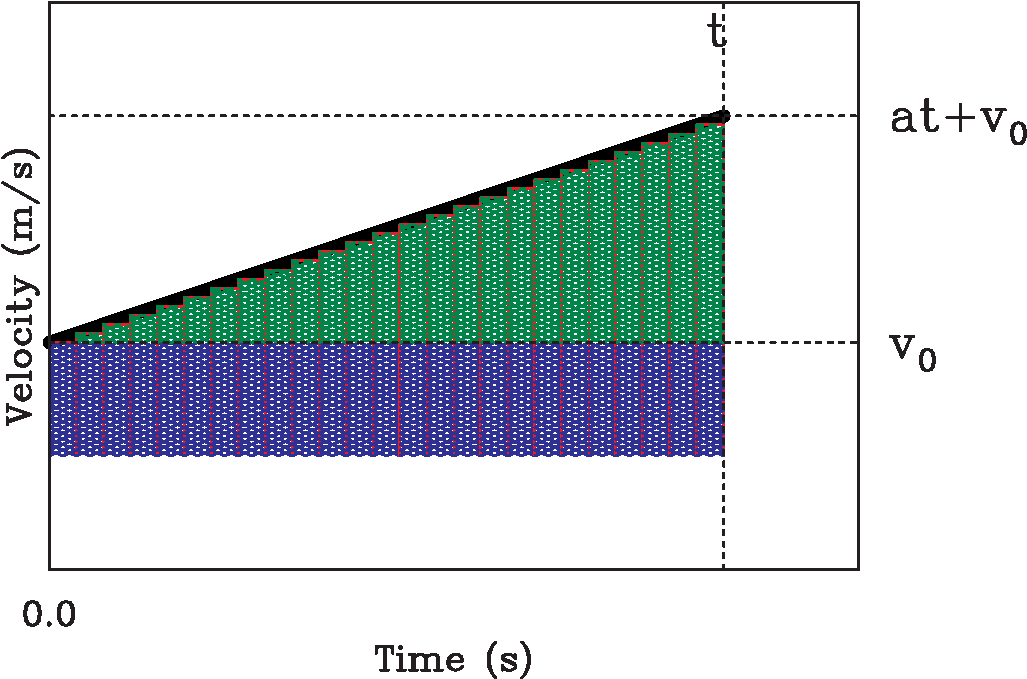
\includegraphics[width=0.6\textwidth]{area-under-v-full-crop.pdf}}

\bigskip

\pause
Area under blue part: $v_0 t$\\
Area under green part: $\frac{1}{2} at^2$\\
Total change in position: $x(t) - x_0 = \frac{1}{2}at^2 + v_0 t$

\bigskip
\bigskip
\centerline{\Large Thus, {\color{Red}$x(t) = \frac{1}{2}at^2 + v_0 t + s_0$}}
}

\frame{\frametitle{\textbf{For those who are familiar with calculus:}}

\begin{align*}
a(t) &= \rm{const}.\\
v(t) &= \int a\,dt &=& at + C_1 \\
x(t) &= \int v\,dt = \int (at + C_1) dt &=& \frac{1}{2}at^2 + C_1 t + C_2
\end{align*}

A little thought reveals that $C_1$ is the initial velocity $v_0$ and $C_2$ is the initial position $x_0$.\\
This gives us the things we just derived, but much more easily:


{\color{Red}
\Large
\begin{align*}
v(t) &=& at + v_0 \\
x(t) &=& \frac{1}{2}at^2 + v_0 t + x_0
\end{align*}}
}

\frame{\frametitle{\textbf{Free fall revisited}}
\centerline{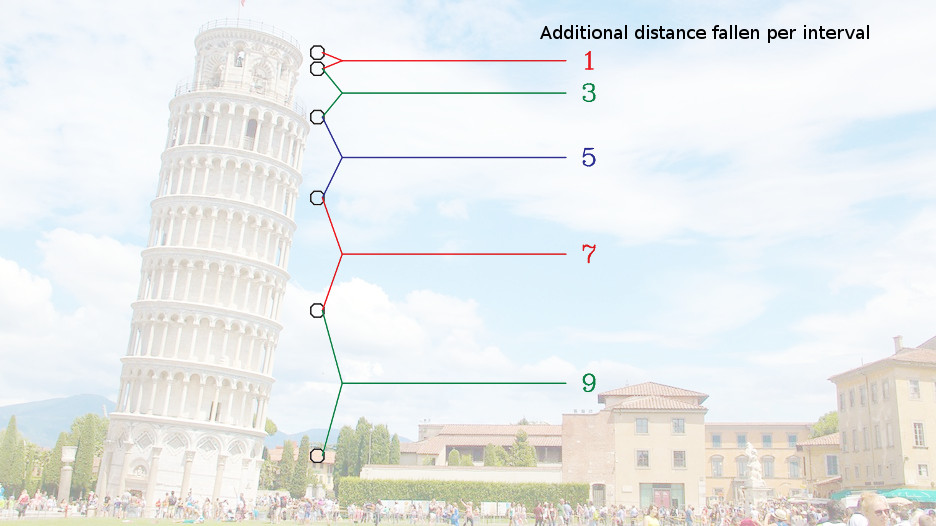
\includegraphics[width=0.8\textwidth]{pisa.jpg}}

\centerline{Adding these numbers together gives us 1, 4, 9, 16, 25...}
\centerline{The calculus above explains this: distance is proportional to {\it time squared!}}
}



\frame{\frametitle{\textbf{Example problems}}
\Large
\BI
\item{How long does it take for a falling object to fall 10 m?}
\EI
}

\frame{\frametitle{\textbf{Example problems}}
\Large
\BI
\item{You throw an object up with an initial speed of $5\, \rm m/\rm s$. How high does it go? How long does it take to come back down?}
\EI
}

\frame{\frametitle{\textbf{Another example}}
\Large 
You throw an object up with an initial speed of $v_0$. How long does it take to reach a height $h$?

\pause

\bigskip

\begin{align*}
x(t) = &\hspace{1.25em}\frac{1}{2}at^2 + v_0 t + x_0 \\
h =& -\frac{1}{2}gt^2 + v_0 t \\
0 =& -\frac{1}{2}gt^2 + v_0 t - h
\end{align*}

\large
\BI
\item{$\rightarrow$ {\color{Red}You need the quadratic formula for this -- nonzero $a$, $v_0$, and position}}
\item{The quadratic formula gives you two answers, but there's clearly only one}
\item{The homework asks you to address this idea.}
\item{Hint: graph position vs. time, and interpret the question graphically}
\EI
}

\frame{\frametitle{\textbf{Rotational kinematics}}
\Large
\BI
\item{Linear motion: care about position as a function of time}
\item{Rotational motion: care about {\color{Red}angle} as a function of time}
\item{\bf Everything we just did translates to rotational kinematics exactly!}
\EI
}

\frame{\frametitle{\textbf{Position, velocity, and acceleration}}
\begin{columns}
\column{0.125\textwidth}
\centerline{\Large Position}
\column{0.2\textwidth}
\small
{\color{Red}
\centerline{(derivative of)}
\centerline{rate of change of}
\centerline{$\xleftarrow{\makebox[\textwidth]{}}$}}
{\color{Green}
\color{Green}\centerline{$\xrightarrow{\makebox[\textwidth]{}}$}}
\color{Green}\centerline{area under the curve of}
\color{Green}\centerline{(integral of)}
\column{0.125\textwidth}
\centerline{\Large Velocity}
\pause
\column{0.2\textwidth}
\small
{\color{Red}
\centerline{(derivative of)}
\centerline{rate of change of}
\centerline{$\xleftarrow{\makebox[\textwidth]{}}$}}
{\color{Green}
\color{Green}\centerline{$\xrightarrow{\makebox[\textwidth]{}}$}}
\color{Green}\centerline{area under the curve of}
\color{Green}\centerline{(integral of)}
\column{0.15\textwidth}
\centerline{\Large Acceleration}
\end{columns}
}

\frame{\frametitle{\textbf{Angle, angular velocity, and angular acceleration}}
\begin{columns}
\column{0.125\textwidth}
\centerline{\Large Angle}
\column{0.2\textwidth}
\small
{\color{Red}
\centerline{(derivative of)}
\centerline{rate of change of}
\centerline{$\xleftarrow{\makebox[\textwidth]{}}$}}
{\color{Green}
\color{Green}\centerline{$\xrightarrow{\makebox[\textwidth]{}}$}}
\color{Green}\centerline{area under the curve of}
\color{Green}\centerline{(integral of)}
\column{0.125\textwidth}
\Large Angular velocity ($\omega$)
\pause
\column{0.2\textwidth}
\small
{\color{Red}
\centerline{(derivative of)}
\centerline{rate of change of}
\centerline{$\xleftarrow{\makebox[\textwidth]{}}$}}
{\color{Green}
\color{Green}\centerline{$\xrightarrow{\makebox[\textwidth]{}}$}}
\color{Green}\centerline{area under the curve of}
\color{Green}\centerline{(integral of)}
\column{0.15\textwidth}
\large Angular acceleration ($\alpha$)
\end{columns}

\Large
\bigskip
\bigskip
\bigskip

\pause

$$ x(t) = x_0 + v_0 t + \frac{1}{2}at^2 $$

$$ \theta(t) = \theta_0 + \omega_0 t + \frac{1}{2}\alpha t^2 $$

\pause

\bigskip

$\rightarrow$ Angular kinematics works in exactly the same way as translational kinematics!

}




\end{document}

